\chapter{Topologias de outros \\ modelos de redes testados}\label{cap:anexo1}
	
	\paragraph{Modelo endógeno MLP\_ENDO\_1}
        O primeiro modelo experimental MLP para obtenção das predições tem topologia definida na figura \ref{fig:case1_mlp_endo1}, denominado MLP\_ENDO\_1, este modelo tem 64 neurônios na primeira camada oculta e 32 neurônios na segunda camada oculta, e assim como todos os outros modelos, 1 neurônio na camada de saída.    
        
        \begin{figure}[h]
        	\center{                		
        	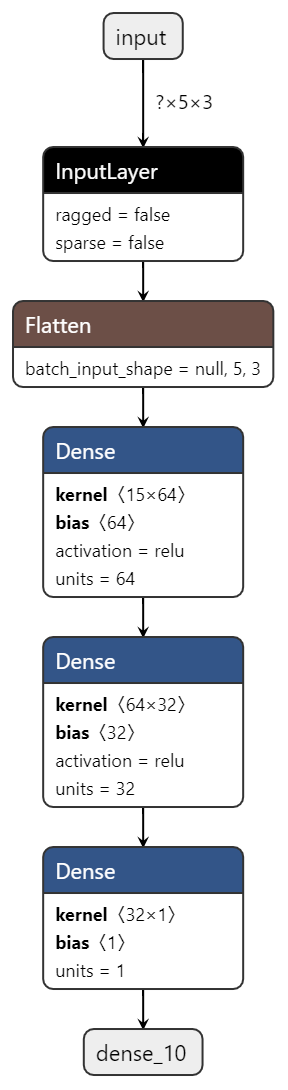
\includegraphics[width=0.4\textwidth]{./Figuras/resultados/case1_mlp_endo1.png}
        	\caption{Topologia do modelo MLP\_ENDO\_1} 
        	\label{fig:case1_mlp_endo1} 
        	}
        \end{figure}
            
    \paragraph{Modelo endógeno GRU RNN\_ENDO\_1}
        Este primeiro modelo experimental GRU foi definido com 16 unidades GRU, com topologia conceitual definida de acordo com a figura \ref{fig:gru-arch} no capítulo de fundamentação teórica \textbf{MLP\_ENDO\_1} e tem um neurônio perpcetron para emissão do sinal de saída, representado pelo bloco \textbf{Dense} na figura \ref{fig:case1_rnn_endo1}
        \begin{figure}[h]
          \center{
            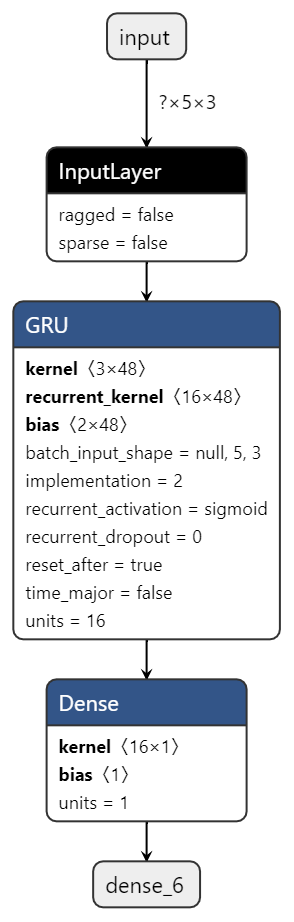
\includegraphics[width=0.4\textwidth]{./Figuras/resultados/case1_rnn_endo1.png}
            \caption{Topologia do modelo RNN\_ENDO\_1} \label{fig:case1_rnn_endo1} }
        \end{figure}
        
        \paragraph{Modelo misto RNN\_EXO\_2}
         O Segundo modelo misto foi definido com o aumento da profundidade das camadas GRU e MLP do modelo anterior, conforme observado na figura \ref{fig:case1_rnn_exo_2} foram acrescentadas 1 camada GRU e 1 camada MLP (Dense).
            \begin{figure}[h]
              \center{
                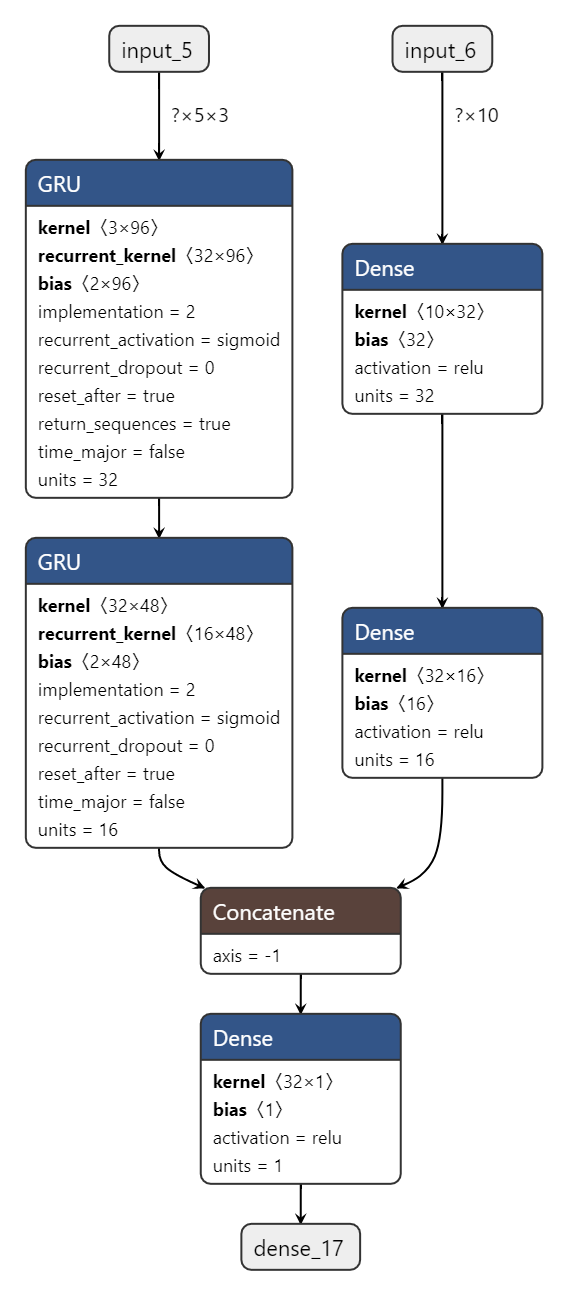
\includegraphics[width=0.6\textwidth]{./Figuras/resultados/case1_rnn_exo_2.png}
              \caption{Topologia do modelo RNN\_EXO\_2}  \label{fig:case1_rnn_exo_2} }
            \end{figure}
        
        \paragraph{Modelo misto RNN\_EXO\_3}
        Para o terceiro e último modelo misto, representado na figura \ref{fig:case1_rnn_exo_3}, foi feita uma reconfiguração do modelo misto anterior, RNN\_EXO\_2, com a utilização do recurso dropout nas saídas das camadas GRU.
        \begin{figure}[h]
          \center{
          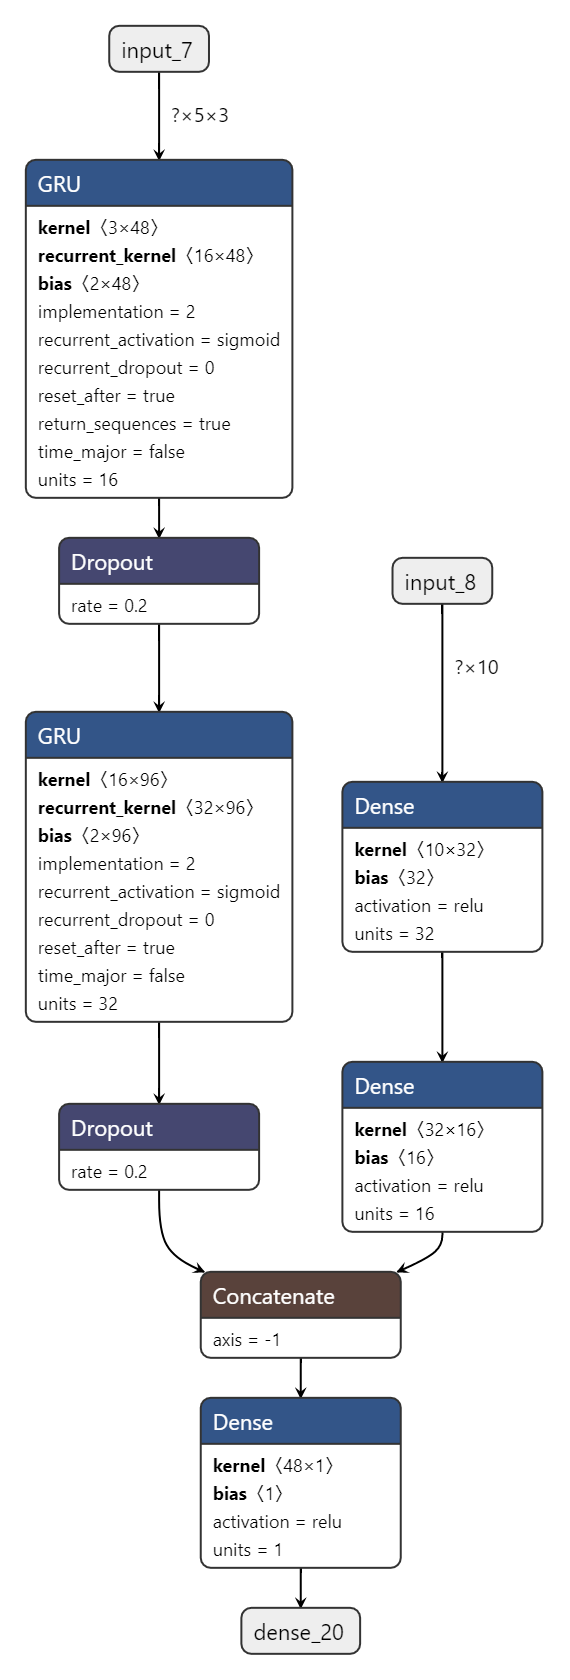
\includegraphics[width=0.5\textwidth]{./Figuras/resultados/case1_rnn_exo_3.png}
          \caption{Topologia do modelo RNN\_EXO\_3} \label{fig:case1_rnn_exo_3} 
          }
        \end{figure}
        

	\chapter{Métodos e códigos experimentais}\label{chapter:outros}

	\section{Primeira Fase Experimental}
	    \paragraph{Pré-Processamento e treino dos modelos}
	        No repositório abaixo, encontram-se os gráficos, métricas e tabelas de todos os modelos treinados na primeira fase experimental, bem como a análise exploratória detalhada de todas as variáveis e parâmetros de entrada nos modelos, e também o detalhamento do pré-processamento dos conjuntos de dados.
	        
	        Os experimentos foram realizados na plataforma Google Colab, em linguagem Python. Nenhuma configuração de ambiente é necessária para reproduzir os experimentos, bastando acessar o link para a plataforma google colab no interior do documento, através de um navegador de internet e executá-los caso seja de interesse.
	        
	        Os experimentos se encontram acessíveis em formato de documento Jupyter Notebook, com recursos de indexação e documentação com blocos de texto e imagens para uma fácil compreensão e acesso instantâneo das informações. \url{https://github.com/ddlandim/monografy-ann-demand-prediction/blob/master/case1__Experimentos_2609.ipynb}
            
	    \paragraph{Importação e aplicação de métricas dos modelos}
	        No link abaixo encontra-se uma página para a importação dos modelos contidos no repositório deste trabalho, já treinados, e encontram-se também o conjuntos de dados pré-processados para o calculo das métricas finais da primeira fase. \url{https://github.com/ddlandim/monografy-ann-demand-prediction/blob/master/case1__ModelsTests_DriverCode.ipynb}
	 
	\section{Segunda Fase Experimental}
	    \paragraph{Pré-Processamento e treino dos modelos}
	        Repositório para os gráficos, métricas e tabelas de todos os modelos treinados na segunda fase experimental. \url{https://github.com/ddlandim/monografy-ann-demand-prediction/blob/master/case2__Experimentos_2709.ipynb}
	    \paragraph{Importação e aplicação de métricas dos modelos}
	         Repositório para a importação dos modelos já treinados e conjuntos de dados já pré-processados para o calculo das métricas finais da segunda fase. \url{https://github.com/ddlandim/monografy-ann-demand-prediction/blob/master/case2__ModelsTests_DriverCode.ipynb}
	        
\section{Tabela completa das métricas de todos os modelos}
        A seguir são listadas as tabelas com todos resultados experimentais.
     
        \begin{table}[!ht]
        \caption{Previsões e erros de todos os modelos}
        \begin{adjustbox}{width=\columnwidth,center}
           \begin{tabular}{ | c | c| c | c| c | }
     \rowcolor{gray!50}
    \multirow{2}{*}{	MODELO} & TOTAL  & TOTAL  & ERRO TOTAL & ERRO TOTAL  \\ \rowcolor{gray!50}
   &                        CONSUMIDAS & PREVISTAS &  PREVISAO &  PERC PREVISAO  \\ 
    \multicolumn{5}{c}{	MODELOS ENDÓGENOS }  \\ \hline
	RNN\_ENDO\_1 1A FASE & 31962 & 30927 & -1035 & -3.2394 \\ \hline
	RNN\_ENDO\_1 2A FASE & 58653 & 60412 & 1759 & 2.9991 \\ \hline
	RNN\_ENDO\_2 1A FASE & 31962 & 31466 & -496 & -1.5530 \\ \hline
	RNN\_ENDO\_2 2A FASE & 58653 & 61855 & 3202 & 5.4594 \\ \hline
	MLP\_ENDO\_1 1A FASE & 31962 & 32370 & 408 & 1.2754 \\ \hline
	MLP\_ENDO\_1 2A FASE & 58653 & 60039 & 1385 & 2.3611 \\ \hline
	\multicolumn{5}{c}{ MODELOS EXÓGENOS }\\ \hline
	RNN\_EXO\_1 1A FASE & 31962 & 28729 & -3233. & -10.1157 \\ \hline
	RNN\_EXO\_1 2A FASE & 58653 & 62048 & 3395 & 5.7883 \\ \hline
	RNN\_EXO\_2 1A FASE & 31962 & 30823 & -1139& -3.5631 \\ \hline
	RNN\_EXO\_2 2A FASE & 58653 & 63161 & 4507 & 7.6849 \\ \hline
	RNN\_EXO\_1 1A FASE & 31962 & 29426 & -2536 & -7.9350 \\ \hline
	RNN\_EXO\_3 2A FASE & 58653 & 58348 & -305 & -0.5196 \\ \hline
	MLP\_ENDO\_1 (**) & 31962 & 31678 & -285 & -0.8901 \\ \hline
	RNN\_EXO\_1 (**) & 31962 & 32170 & 208 & 0.6515 \\ \hline
\end{tabular} \end{adjustbox}\caption*{(**) \textbf{MODELOS TREINADOS NA 2A FASE E TESTADOS NO DOMÍNIO DA 1A FASE}} \end{table} 

\begin{table}[!ht]
        \caption{Erros quantitativos de todos os modelos}
        \begin{adjustbox}{width=\columnwidth,center}
           \begin{tabular}{ | c | c| c | c| c | }
     \rowcolor{gray!50}
    \multirow{2}{*}{	MODELO} & TOTAL SOMA  & TOTAL SOMA  & ERRO ABS & ERRO ABS \\ \rowcolor{gray!50}
   &                         ERROS POSITIVOS &  ERROS NEGATIVOS &  MEDIANO&  PERC MEDIO \\ 
    \multicolumn{5}{c}{	MODELOS ENDÓGENOS }  \\ \hline
RNN\_ENDO\_1 1A FASE & -3281 & 4316 & 74.0192 & 87.4987 \\ \hline
	RNN\_ENDO\_1 2A FASE & -7709 & 5950 & 58.4248 & 107.8793 \\ \hline
	RNN\_ENDO\_2 1A FASE & -2983 & 3479 & 46.7072 & 74.9353 \\ \hline
	RNN\_ENDO\_2 2A FASE & -8335 & 5133. & 55.7799 & 101.2846 \\ \hline
	MLP\_ENDO\_1 1A FASE & -4306 & 3898 & 71.8950 & 92.5815 \\ \hline
	MLP\_ENDO\_1 2A FASE & -7097 & 5712 & 53.8804 & 98.5516 \\ \hline
	\multicolumn{5}{c}{ MODELOS EXÓGENOS }\\ \hline
RNN\_EXO\_1 1A FASE & -2709 & 5942 & 85.5910 & 90.9869 \\ \hline
	RNN\_EXO\_1 2A FASE & -8163 & 4768 & 55.2355 & 224.9068 \\ \hline
	RNN\_EXO\_2 1A FASE & -3045 & 4184 & 63.5989 & 88.2687 \\ \hline
	RNN\_EXO\_2 2A FASE & -9677 & 5170 & 64.6863 & 230.9423 \\ \hline
	RNN\_EXO\_1 1A FASE & -3418 & 5954 & 100.4442 & 98.7906 \\ \hline
	RNN\_EXO\_3 2A FASE & -8608 & 8913 & 85.1866 & 236.5670 \\ \hline
	MLP\_ENDO\_1(**) & -351 & 3797 & 65.6641 & 84.9684 \\ \hline
	RNN\_EXO\_1  (**) & -3455 & 3247 & 59.5414 & 83.2671\\ \hline
\end{tabular} \end{adjustbox}\caption*{(**) \textbf{MODELOS TREINADOS NA 2A FASE E TESTADOS NO DOMÍNIO DA 1A FASE}} \end{table} 

	    \begin{table}[!ht]
        \caption{Métricas estatísticas e de treino de todos os modelos}
        \begin{adjustbox}{width=0.8\columnwidth,center}
           \begin{tabular}{ |c | c| c | c| }
     \rowcolor{gray!50}
   {	MODELO} & r\_2 value &	std\_err & RMSE \\ \hline
     \multicolumn{4}{c}{	MODELOS ENDÓGENOS }  \\ \hline
RNN\_ENDO\_1 1A FASE&	0,2277	&0,0600&	115,5925\\ \hline
RNN\_ENDO\_1 2A FASE&	0,4034	&0,0417&	101,1817\\ \hline
RNN\_ENDO\_2 1A FASE&	0,3545	&0,0721&	108,0663\\ \hline
RNN\_ENDO\_2 2A FASE&	0,3933	&0,0474&	105,3284\\ \hline
MLP\_ENDO\_1 1A FASE&	0,2716	&0,0947&	128,0541\\ \hline
MLP\_ENDO\_1 2A FASE&	0,4354	&0,0484&	101,1515\\ \hline
	\multicolumn{4}{c}{ MODELOS EXÓGENOS }\\ \hline
RNN\_EXO\_1 1A FASE &	0,1699 &		0,0551 &		124,4907\\ \hline
RNN\_EXO\_1 2A FASE &	0,4508 &		0,0445 &		 99,3650\\ \hline
RNN\_EXO\_2 1A FASE &	0,2710 &		0,0639 &		112,9921\\ \hline
RNN\_EXO\_2 2A FASE &	0,3539 &		0,0417 &		107,8493\\ \hline
RNN\_EXO\_1 1A FASE &	0,1153 &		0,0306 &		124,6581\\ \hline
RNN\_EXO\_3 2A FASE &	0,1953 &		0,0366 &		117,0316\\ \hline
MLP\_ENDO\_1 (**)   &   0,2896 &		0,0788 &		116,6204\\ \hline
RNN\_EXO\_1  (**)   &	0,3485 &		0,0658 &		106,2080\\ \hline
\end{tabular} \end{adjustbox}\caption*{(**) \textbf{MODELOS TREINADOS NA 2A FASE E TESTADOS NO DOMÍNIO DA 1A FASE}} \end{table} 
	    
\begin{table}[!ht]
        \caption{Métricas gráficas de todos os modelos}
        \begin{adjustbox}{width=\columnwidth,center}
           \begin{tabular}{ | c | c| c | c| c |}
     \rowcolor{gray!50}
   {	MODELO} & CORRELAÇÂO &	p-value &	slope & 	intercept\\ \hline
     \multicolumn{5}{c}{	MODELOS ENDÓGENOS }  \\ \hline
RNN\_ENDO\_1 1A FASE &	0,4772&		2,5815E-06&		0,3022&		241,6487 \\ \hline
RNN\_ENDO\_1 2A FASE&	0,6351&		5,9900E-22&		0,4601&		183,6360\\ \hline
RNN\_ENDO\_2 1A FASE&	0,5954&		9,4221E-10&		0,4956&		177,5496\\ \hline
RNN\_ENDO\_2 2A FASE&	0,6271&		2,7285E-21&		0,5125&		174,6988\\ \hline
MLP\_ENDO\_1 1A FASE&	0,5212&		1,9211E-07&		0,5365&		172,9566\\ \hline
MLP\_ENDO\_1 2A FASE&	0,6599&		3,9898E-24&		0,5704&		146,0429\\ \hline
	\multicolumn{5}{c}{ MODELOS EXÓGENOS }\\ \hline
RNN\_EXO\_1 1A FASE&	0,4122&		6,5907E-05&		0,2313&		242,4375 \\ \hline
RNN\_EXO\_1 2A FASE&	0,6714&		3,2984E-25&		0,5421&		166,2111 \\ \hline
RNN\_EXO\_2 1A FASE&	0,5206&		1,9952E-07&		0,3613&		219,0125 \\ \hline
RNN\_EXO\_2 2A FASE&	0,5948&		8,3516E-19&		0,4149&		213,3027 \\ \hline
RNN\_EXO\_1 1A FASE&	0,3396&		0,00126742&		0,1025&		297,1444 \\ \hline
RNN\_EXO\_3 2A FASE&	0,4419&		4,2231E-10&		0,2424&		242,4514 \\ \hline
MLP\_ENDO\_1 (**)&		0,5382&		6,36258E-08&	0,4668&		190,4162 \\ \hline
RNN\_EXO\_1  (**)&		0,5903&		1,41433E-09&	0,4468&		203,2738 \\ \hline
\end{tabular} \end{adjustbox} \caption*{(**) \textbf{MODELOS TREINADOS NA 2A FASE E TESTADOS NO DOMÍNIO DA 1A FASE}}\end{table} 